% Options for packages loaded elsewhere
% Options for packages loaded elsewhere
\PassOptionsToPackage{unicode}{hyperref}
\PassOptionsToPackage{hyphens}{url}
\PassOptionsToPackage{dvipsnames,svgnames,x11names}{xcolor}
%
\documentclass[
]{fypStandard}
\usepackage{xcolor}
\usepackage{amsmath,amssymb}
\setcounter{secnumdepth}{4}
\usepackage{iftex}
\ifPDFTeX
  \usepackage[T1]{fontenc}
  \usepackage[utf8]{inputenc}
  \usepackage{textcomp} % provide euro and other symbols
\else % if luatex or xetex
  \usepackage{unicode-math} % this also loads fontspec
  \defaultfontfeatures{Scale=MatchLowercase}
  \defaultfontfeatures[\rmfamily]{Ligatures=TeX,Scale=1}
\fi
\usepackage{lmodern}
\ifPDFTeX\else
  % xetex/luatex font selection
\fi
% Use upquote if available, for straight quotes in verbatim environments
\IfFileExists{upquote.sty}{\usepackage{upquote}}{}
\IfFileExists{microtype.sty}{% use microtype if available
  \usepackage[]{microtype}
  \UseMicrotypeSet[protrusion]{basicmath} % disable protrusion for tt fonts
}{}
\makeatletter
\@ifundefined{KOMAClassName}{% if non-KOMA class
  \IfFileExists{parskip.sty}{%
    \usepackage{parskip}
  }{% else
    \setlength{\parindent}{0pt}
    \setlength{\parskip}{6pt plus 2pt minus 1pt}}
}{% if KOMA class
  \KOMAoptions{parskip=half}}
\makeatother
% Make \paragraph and \subparagraph free-standing
\makeatletter
\ifx\paragraph\undefined\else
  \let\oldparagraph\paragraph
  \renewcommand{\paragraph}{
    \@ifstar
      \xxxParagraphStar
      \xxxParagraphNoStar
  }
  \newcommand{\xxxParagraphStar}[1]{\oldparagraph*{#1}\mbox{}}
  \newcommand{\xxxParagraphNoStar}[1]{\oldparagraph{#1}\mbox{}}
\fi
\ifx\subparagraph\undefined\else
  \let\oldsubparagraph\subparagraph
  \renewcommand{\subparagraph}{
    \@ifstar
      \xxxSubParagraphStar
      \xxxSubParagraphNoStar
  }
  \newcommand{\xxxSubParagraphStar}[1]{\oldsubparagraph*{#1}\mbox{}}
  \newcommand{\xxxSubParagraphNoStar}[1]{\oldsubparagraph{#1}\mbox{}}
\fi
\makeatother


\usepackage{longtable,booktabs,array}
\usepackage{calc} % for calculating minipage widths
% Correct order of tables after \paragraph or \subparagraph
\usepackage{etoolbox}
\makeatletter
\patchcmd\longtable{\par}{\if@noskipsec\mbox{}\fi\par}{}{}
\makeatother
% Allow footnotes in longtable head/foot
\IfFileExists{footnotehyper.sty}{\usepackage{footnotehyper}}{\usepackage{footnote}}
\makesavenoteenv{longtable}
\usepackage{graphicx}
\makeatletter
\newsavebox\pandoc@box
\newcommand*\pandocbounded[1]{% scales image to fit in text height/width
  \sbox\pandoc@box{#1}%
  \Gscale@div\@tempa{\textheight}{\dimexpr\ht\pandoc@box+\dp\pandoc@box\relax}%
  \Gscale@div\@tempb{\linewidth}{\wd\pandoc@box}%
  \ifdim\@tempb\p@<\@tempa\p@\let\@tempa\@tempb\fi% select the smaller of both
  \ifdim\@tempa\p@<\p@\scalebox{\@tempa}{\usebox\pandoc@box}%
  \else\usebox{\pandoc@box}%
  \fi%
}
% Set default figure placement to htbp
\def\fps@figure{htbp}
\makeatother


% definitions for citeproc citations
\NewDocumentCommand\citeproctext{}{}
\NewDocumentCommand\citeproc{mm}{%
  \begingroup\def\citeproctext{#2}\cite{#1}\endgroup}
\makeatletter
 % allow citations to break across lines
 \let\@cite@ofmt\@firstofone
 % avoid brackets around text for \cite:
 \def\@biblabel#1{}
 \def\@cite#1#2{{#1\if@tempswa , #2\fi}}
\makeatother
\newlength{\cslhangindent}
\setlength{\cslhangindent}{1.5em}
\newlength{\csllabelwidth}
\setlength{\csllabelwidth}{3em}
\newenvironment{CSLReferences}[2] % #1 hanging-indent, #2 entry-spacing
 {\begin{list}{}{%
  \setlength{\itemindent}{0pt}
  \setlength{\leftmargin}{0pt}
  \setlength{\parsep}{0pt}
  % turn on hanging indent if param 1 is 1
  \ifodd #1
   \setlength{\leftmargin}{\cslhangindent}
   \setlength{\itemindent}{-1\cslhangindent}
  \fi
  % set entry spacing
  \setlength{\itemsep}{#2\baselineskip}}}
 {\end{list}}
\usepackage{calc}
\newcommand{\CSLBlock}[1]{\hfill\break\parbox[t]{\linewidth}{\strut\ignorespaces#1\strut}}
\newcommand{\CSLLeftMargin}[1]{\parbox[t]{\csllabelwidth}{\strut#1\strut}}
\newcommand{\CSLRightInline}[1]{\parbox[t]{\linewidth - \csllabelwidth}{\strut#1\strut}}
\newcommand{\CSLIndent}[1]{\hspace{\cslhangindent}#1}



\setlength{\emergencystretch}{3em} % prevent overfull lines

\providecommand{\tightlist}{%
  \setlength{\itemsep}{0pt}\setlength{\parskip}{0pt}}



 


% ===================================================================
% PROJECT METADATA — Edit these values for your project
% ===================================================================
\projectid{FYP01-IS-T2510-0001}
\projecttitle{Your Approved Project Title Goes Here}
\studentid{1234567890}
\studentname{YOUR FULL NAME}
\programme{BACHELOR OF INFORMATION TECHNOLOGY}
\degreename{BACHELOR OF INFORMATION TECHNOLOGY}
\submissionmonthyear{JUNE 2026}
\submissionyear{2026}
\reporttype{INTERIM}
\supervisorname{Dr. Supervisor Name}
\makeatletter
\@ifpackageloaded{caption}{}{\usepackage{caption}}
\AtBeginDocument{%
\ifdefined\contentsname
  \renewcommand*\contentsname{Table of contents}
\else
  \newcommand\contentsname{Table of contents}
\fi
\ifdefined\listfigurename
  \renewcommand*\listfigurename{List of Figures}
\else
  \newcommand\listfigurename{List of Figures}
\fi
\ifdefined\listtablename
  \renewcommand*\listtablename{List of Tables}
\else
  \newcommand\listtablename{List of Tables}
\fi
\ifdefined\figurename
  \renewcommand*\figurename{Figure}
\else
  \newcommand\figurename{Figure}
\fi
\ifdefined\tablename
  \renewcommand*\tablename{Table}
\else
  \newcommand\tablename{Table}
\fi
}
\@ifpackageloaded{float}{}{\usepackage{float}}
\floatstyle{ruled}
\@ifundefined{c@chapter}{\newfloat{codelisting}{h}{lop}}{\newfloat{codelisting}{h}{lop}[chapter]}
\floatname{codelisting}{Listing}
\newcommand*\listoflistings{\listof{codelisting}{List of Listings}}
\makeatother
\makeatletter
\makeatother
\makeatletter
\@ifpackageloaded{caption}{}{\usepackage{caption}}
\@ifpackageloaded{subcaption}{}{\usepackage{subcaption}}
\makeatother
\usepackage{bookmark}
\IfFileExists{xurl.sty}{\usepackage{xurl}}{} % add URL line breaks if available
\urlstyle{same}
\hypersetup{
  colorlinks=true,
  linkcolor={blue},
  filecolor={Maroon},
  citecolor={Blue},
  urlcolor={Blue},
  pdfcreator={LaTeX via pandoc}}


\author{}
\date{}
\begin{document}

% ===================================================================
% PRELIMINARY PAGES (Cover, Title, Copyright, Declaration, etc.)
% ===================================================================

% -- Cover Page --
\makecoverpage

% -- Title Page --
\maketitlepage

% -- Switch to Roman numeral page numbering for preliminary pages --
\frontmatteraliased

% -- Copyright Page --
\makecopyrightpage

% -- Declaration Page --
\makedeclarationpage

% -- Acknowledgements --
\begin{acknowledgements}
I would like to express my sincere gratitude to my supervisor,
for the continuous guidance and support throughout this project.

I would also like to thank the Faculty of Computing and Informatics,
Multimedia University, for providing the resources and environment
necessary to complete this work.

Finally, I am grateful to my family and friends for their
encouragement and understanding.
\end{acknowledgements}

% -- Abstract --
\begin{abstract}
Write your abstract here. In one page, certainly not more than two,
summarize the main features of your project; describe what problem
you are solving and how you propose to solve it. This brief overview
should give a snapshot of the overall structure of your final year
project.
\end{abstract}

% -- Table of Contents (manually generated in prelim pages) --
\renewcommand*\contentsname{TABLE OF CONTENTS}
{
\hypersetup{linkcolor=black}
\setcounter{tocdepth}{3}
\tableofcontents
}

% -- List of Tables --
\listoftables

% -- List of Figures --
\listoffigures

% -- List of Abbreviations (add your abbreviations below) --
\begin{listofabbreviations}
\begin{tabular}{@{}ll@{}}
API   & Application Programming Interface \\
FYP   & Final Year Project \\
MMU   & Multimedia University \\
FCI   & Faculty of Computing and Informatics \\
UML   & Unified Modeling Language \\
\end{tabular}
\end{listofabbreviations}

% -- List of Appendices --
\begin{listofappendices}
\begin{tabular}{@{}ll@{}}
Appendix A & Gantt Chart \\
Appendix B & FYP I Meeting Logs \\
Appendix C & Turnitin Similarity Index Page \\
\end{tabular}
\end{listofappendices}

% ===================================================================
% SWITCH TO MAIN MATTER (Arabic page numbering starts at 1)
% ===================================================================
\mainmatteraliased


\chapter{Introduction}\label{introduction}

\section{Overview}\label{overview}

Provide an overview description of the project. How did the problem
present itself to you in the first place? Describe the nature of the
problem in detail.

\section{Problem Statement}\label{problem-statement}

Clearly define the problem that this project aims to address. Explain
the context and significance of the problem.

\begin{figure}[H]

{\centering \pandocbounded{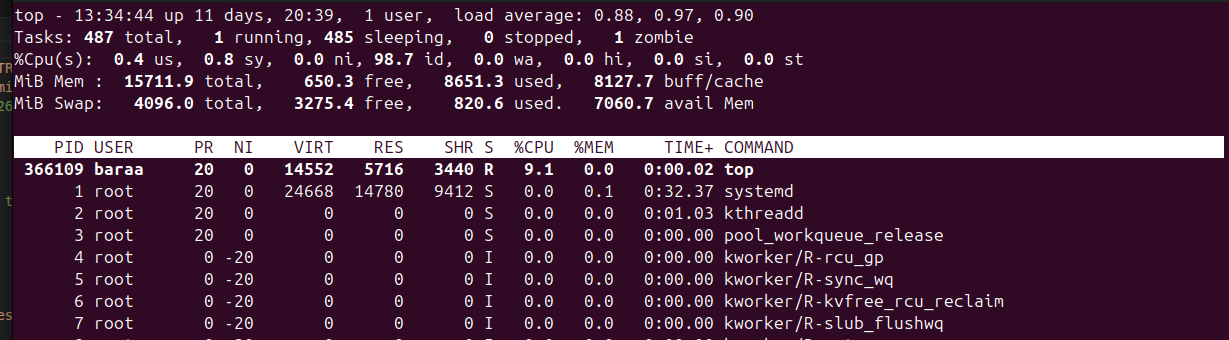
\includegraphics[keepaspectratio]{images/example.png}}

}

\caption{example figure}

\end{figure}%

\section{Project Objectives}\label{project-objectives}

The objectives of this project are as follows:

\begin{enumerate}
\def\labelenumi{\arabic{enumi}.}
\tightlist
\item
  First objective.
\item
  Second objective.
\item
  Third objective.
\end{enumerate}

\section{Project Scope}\label{project-scope}

Define the boundaries of your project. What will be covered and what
will not be covered.

\section{Project Limitations}\label{project-limitations}

Describe any known limitations or constraints of the project.

\section{Methodology}\label{methodology}

Briefly describe the methodology or approach that will be used in this
project.

\section{Target Audience}\label{target-audience}

Describe who will benefit from or use the outcome of this project.

\section{Summary}\label{summary}

Summarize the key points covered in this chapter and provide a brief
overview of the remaining chapters.

\chapter{Literature Review}\label{literature-review}

\section{Overview}\label{overview-1}

This chapter presents a comprehensive review of existing literature
related to the project topic.

\section{Topic Title}\label{topic-title}

\subsection{Sub-topic}\label{sub-topic}

Discuss relevant literature, prior work, and existing solutions related
to your project.

\begin{longtable}[]{@{}ll@{}}
\caption{example table of commands}\tabularnewline
\toprule\noalign{}
example & table \\
\midrule\noalign{}
\endfirsthead
\toprule\noalign{}
example & table \\
\midrule\noalign{}
\endhead
\bottomrule\noalign{}
\endlastfoot
\textbf{Newest logs first} & \texttt{journalctl\ -r} \\
\textbf{Current boot only} & \texttt{journalctl\ -b} \\
\textbf{Follow live (real-time)} & \texttt{journalctl\ -f} \\
\textbf{Specific service} &
\texttt{journalctl\ -u\ \textless{}Service\ Name\textgreater{}} \\
\textbf{Show last 50 lines} & \texttt{journalctl\ -n\ 50} \\
\end{longtable}

\section{Summary}\label{summary-1}

Summarize the key findings from the literature review and identify the
research gap.

\chapter{Requirements Analysis}\label{requirements-analysis}

\section{Overview}\label{overview-2}

This chapter describes the requirements gathering techniques and
analysis of results.

\section{Fact-Finding Techniques}\label{fact-finding-techniques}

\subsection{Justification}\label{justification}

Justify the choice of fact-finding techniques used.

\subsection{Questionnaire Design}\label{questionnaire-design}

\subsubsection{Analysis on Results}\label{analysis-on-results}

Present and analyse the results of any questionnaires conducted.

\subsection{Observation}\label{observation}

\subsubsection{Analysis on Results}\label{analysis-on-results-1}

Present and analyse the results of any observations conducted.

\section{Requirements}\label{requirements}

\subsection{Functional Requirements}\label{functional-requirements}

List and describe the functional requirements of the system.

\subsection{Non-functional
Requirements}\label{non-functional-requirements}

List and describe the non-functional requirements of the system.

\subsection{User Requirements}\label{user-requirements}

Describe the user requirements gathered from stakeholders.

\chapter{System Design}\label{system-design}

\section{Overview}\label{overview-3}

This chapter presents the system design for the proposed solution.

\section{Rich Picture Diagram}\label{rich-picture-diagram}

Include and describe the rich picture diagram.

\section{Use Case Diagram}\label{use-case-diagram}

Include and describe the use case diagram.

\section{Activity Diagram}\label{activity-diagram}

Include and describe the activity diagram.

\section{Class Diagram}\label{class-diagram}

Include and describe the class diagram.

\section{Sequence Diagram}\label{sequence-diagram}

Include and describe the sequence diagram.

\section{Interface Design}\label{interface-design}

Present the interface designs and mockups.

\section{Summary}\label{summary-2}

Summarize the system design decisions made.

\chapter{Implementation Plan}\label{implementation-plan}

\section{Development Phase}\label{development-phase}

Describe the front-end and back-end coding plan.

\section{Testing Phase}\label{testing-phase}

Describe the testing strategy: unit testing, integration testing, system
testing, and user acceptance testing (UAT).

\section{Deployment Phase}\label{deployment-phase}

Describe the deployment plan, if applicable.

\chapter{Conclusion}\label{conclusion}

Summarize what has been achieved related to the objectives, and what is
to be achieved in the next phase of the project. Describe any issues
experienced during the project such as problems encountered.

\newpage

\chapter*{References}\label{references}
\addcontentsline{toc}{chapter}{References}

\phantomsection\label{refs}
\begin{CSLReferences}{1}{0}
\bibitem[\citeproctext]{ref-sample2024}
Smith, J. A., \& Jones, M. B. (2024). A sample reference entry for
demonstration purposes. \emph{Journal of Computing and Informatics},
\emph{10}(2), 100--115. \url{https://doi.org/10.1234/jci.2024.0001}

\end{CSLReferences}

\newpage
\appendix

\chapter*{Gantt Chart}\label{gantt-chart}
\addcontentsline{toc}{chapter}{Gantt Chart}

\addcontentsline{toc}{chapter}{Appendix A: Gantt Chart}

Replace this text with your Gantt chart using one of the options above.

\newpage

\chapter*{FYP I Meeting Logs}\label{fyp-i-meeting-logs}
\addcontentsline{toc}{chapter}{FYP I Meeting Logs}

\addcontentsline{toc}{chapter}{Appendix B: FYP I Meeting Logs}

Replace this text with your meeting logs using one of the options above.
A minimum of six (6) meeting logs are required.

\newpage

\chapter*{Turnitin Similarity Index
Page}\label{turnitin-similarity-index-page}
\addcontentsline{toc}{chapter}{Turnitin Similarity Index Page}

\addcontentsline{toc}{chapter}{Appendix C: Turnitin Similarity Index Page}

Replace this text with your Turnitin report using one of the options
above. Overall Similarity Index must be \(\leq\) 20\%.




\end{document}
